\documentclass[border=3mm]{standalone}
\usepackage{ifpdf}
\usepackage[table]{xcolor}
\definecolor{dnvang}{HTML}{E5890A}
\definecolor{dnxanh}{HTML}{3A98B9}
\definecolor{dnxanhdam}{HTML}{19376D}
\definecolor{dndo}{HTML}{BB2649}
\definecolor{dntim}{HTML}{5B0888}
\def\mycolor{dnvang}
\def\mauphu{dntim!80!black}
\def\maudam{dnxanhdam}
\def\maunhan{dndo}
\pagestyle{empty}
\usepackage[utf8]{vietnam}
\usepackage{tikz}
\usetikzlibrary{shapes,calc}
\usepackage{xparse}
\newif\ifWithNames\WithNamestrue
%%%%%
\newcommand{\NTDTextFormat}[4]
{
	\begin{minipage}{2.2cm}
		\centering
		{\textbf{#1} \hfill #2}%
		\linebreak \linebreak
		{\textbf{#3}}%
		\linebreak \linebreak
		{\ifWithNames\large {#4}\fi}
	\end{minipage}
}

\newcommand{\NTDElement}[4]
{
	\NTDTextFormat{\color{white}{\Large#1}}{\color{white}{\Large #2}}{\color{white}\LARGE {#3}}{\color{white}\Large#4}
}
\newcommand{\OutlineText}[1]
{
	\ifpdf
	\pdfliteral direct {0.5 w 1 Tr}{#1}%
	\pdfliteral direct {1 w 0 Tr}%
	\else
	\pscharpath[shadow=false,
	fillstyle=solid,
	fillcolor=white,
	linestyle=solid,
	linecolor=black,
	linewidth=.2pt]{#1}
	\fi
}

\newcommand{\OutlineElement}[4]
{
	\ifpdf
	\NTDElement{\color{white}{\Large#1}}{\color{white}{\Large#2}}{\OutlineText{\LARGE \color{white}{\Large#3}}}{\color{white}{\Large#4}}
	\else
	\NTDElement{\Large#1}{\Large#2}{\OutlineText{\LARGE #3}}{\Large#4}
	\fi
}
\tikzstyle{NTDFill} = [fill=\mauphu!90]
\tikzstyle{NTD} = [draw=white, NTDFill,
minimum width=3.5cm, minimum height=3.5cm, node distance=3.7cm,rounded corners =3pt]
%%%%%%%%%%%%%%%%%%%%%%%%%%%%%%%%%%%%%%%%%%%%%%%%%%%%%%%%%%%%%%%%%%%%%%%%%%%%%%%%%%%%
\begin{document}
	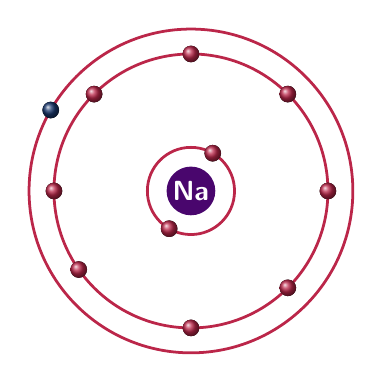
\begin{tikzpicture}[declare function ={r1=35pt;r2=110pt;r3=130pt;r4=243pt;r5=265pt;r6=298pt;k=.45;}]
		\path (0:0) coordinate (O);
		\draw[\maunhan,line width=1pt] 
		(O) circle (k*r3) 
		(O) circle (k*r2) 
		(O) circle (k*r1)
		;
		\path (O) node [shape =circle , inner sep =1pt,font=\color{white}\bfseries\sffamily,fill=\mauphu]{Na};
		\path (60:k*r1) node {\tikz{\fill[ball color =\maunhan] circle(3pt);}}
		(240:k*r1) node {\tikz{\fill[ball color =\maunhan] circle(3pt);}}
		(90:k*r2) node {\tikz{\fill[ball color =\maunhan] circle(3pt);}}
		(-90:k*r2) node {\tikz{\fill[ball color =\maunhan] circle(3pt);}}
		(0:k*r2) node {\tikz{\fill[ball color =\maunhan] circle(3pt);}}
		(180:k*r2) node {\tikz{\fill[ball color =\maunhan] circle(3pt);}}
		(135:k*r2) node {\tikz{\fill[ball color =\maunhan] circle(3pt);}}
		(-45:k*r2) node {\tikz{\fill[ball color =\maunhan] circle(3pt);}}
		(45:k*r2) node {\tikz{\fill[ball color =\maunhan] circle(3pt);}}
		(215:k*r2) node {\tikz{\fill[ball color =\maunhan] circle(3pt);}}
		(-210:k*r3) node {\tikz{\fill[ball color =\maudam] circle(3pt);}}
		;
		
	\end{tikzpicture}
\end{document}